\chapter{Combined Analysis of {\eedm} and {\nedm}}
\label{ch:combined-eEDM-nEDM}

In the previous two chapters, we saw that our {\gthdm} predictions for {\eedm} and {\nedm} lie either right on or slighly below their current respective experimental bounds.
This strongly suggests that the combined results of these two observables will hold great significance,
and is warrant of a combined analysis and discussion.
We present combined results for {\eedm} and {\nedm} with the extended cancellation ansatz~\eqnref{eq:ansatz-extended} in the range \(r \in [0.6, 0.8] \) in \figref{fig:nEDM-eEDM}.
The {\eedm} cancellation mechanism from \secref{sec:eEDM-cancellation} at \(r \approx 0.7 \) is clearly illustrated,
while {\nedm} exhibits no obvious cancellation phenomena.
If one were to isolate the EDM contributions of the individual up and down quarks,
the ansatz-based cancellation would indeed occur seperately for each quark.
However, the chromo-EDM and Weinberg diagram contributions do not exhibit this kind of cancellation,
so there is no visible cancellation for {\nedm}.
For the relaxed ``order-of-magnitude'' \(\rho_{uu} \), we refer back to \figref{fig:nEDM-varied}.
Since \(\rho_{uu} \) does not meaningfully contribute to \(d_{e} \), 
the {\eedm} parameter space is not significantly affected by this relaxation of the ansatz.
If one looks closely, one can see points of the same color forming the signature ``cancellation dip'' in the {\eedm} direction.
This also elucidates that the \emph{natural} cancellation in {\nedm} is a different mechanism from the \emph{ansatz-based} cancellation of {\eedm}.

To apply our theoretical predictions, we turn our gaze toward the {\eedm} and {\nedm} experiments.
Given the recent rapid development on the {\eedm} experimental front, 
it is not unreasonable to expect an order-of-magnitude improvement in the coming decade.
As mentioned in \secref{sec:nEDM_experimentalOverview}, 
n2EDM at PSI projects an order-of-magnitude increase in precision in the next decade,
while SNS at ORNL projects a two-order-of-magnitude increase in precision in the next 20 years.
This means that within the two decades to come,
both the {\eedm} and {\nedm} experimental fronts will have enough precision to probe the vast majority of our respective predicted {\gthdm} parameter spaces.
This puts {\gthdm} in the prime position for \emph{discovery} in not one, but TWO precision fronts.
One could even call that a \emph{double whammy}!
However, given the pretty specific conditions proposed for {\eedm}, 
resulting in a rather restrictive parameter space,
one might deem our hope of discovery right around the current bound at \num{e-30}, or even \num{e-29},
to be wishful thinking.
We would then refer you to the story of the discovery of \(B_{0} - \bar{B_{0}} \) mixing.
In 1987, CLEO~\cite{CLEO1987BBbarMixing} published their bound on the strength of \(B_{0} - \bar{B_{0}} \).
In that same year, ARGUS~\cite{ARGUS1987BBbarMixing} announced their \emph{discovery} of \(B_{0} - \bar{B_{0}} \) right on the CLEO bound.
Thus, it is not unreasonable to expect an {\eedm} discovery in the vicinity of the current JILA bound.

\clearpage
% Combined nEDM-eEDM fixed rho_uu
\begin{figure}[p]
  \centering
  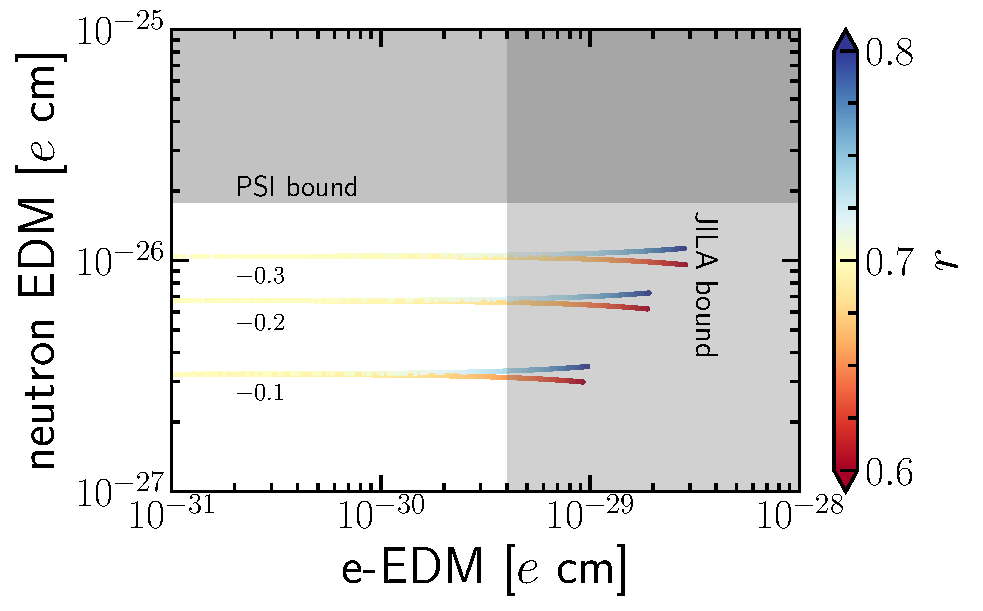
\includegraphics[width=0.8\linewidth]{fig3.pdf}
  \caption{Combined eEDM-nEDM results.}
  \label{fig:nEDM-eEDM}
\end{figure}